% !TeX spellcheck = it_IT

\documentclass[9pt, format=169]{beamer}

\usepackage[utf8]{inputenc}
\usepackage[italian]{babel}
\usepackage{multicol}

\usetheme{metropolis}

\usepackage{mathtools}
\DeclarePairedDelimiter{\ceil}{\lceil}{\rceil}

\title{Esercitazioni di Informatica B}
\subtitle{Codifica dell'informazione}

\author{Stefano Cereda\\
	stefano.cereda@polimi.it
}
\date{02/10/2018 e 08/10/2018}
\institute[PoliMi]{\vspace{0.5cm}\centering Politecnico di Milano \\ \vspace{0.2cm}
	
\includegraphics[width=0.2\textwidth]{../logopolimi}}

\setbeamercovered{invisible}

\makeindex

\begin{document}
	\begin{frame}
	\maketitle
	\end{frame}

	\begin{frame}<handout:0>{}
		\Huge{Settimana prossima ci sarà solamente esercitazione il lunedì mattina.}
	\end{frame}

	\begin{frame}{Argomenti}
	\tableofcontents
	\end{frame}

\section{Codifiche}

\begin{frame}{Alfabeti e codifiche}
Una codifica è una regola arbitraria che consente di dare un significato a dei simboli.

L'insieme di simboli (e.g. cifre) utilizzabili definisce l'alfabeto.

\pause
Dato un alfabeto con $S$ simboli, le possibili combinazioni di lunghezza $L$ sono $C = S^L$.

Viceversa, per rappresentare $C$ combinazioni tramite un alfabeto di $S$ simboli avremo bisogno di combinazioni di lunghezza $L = \ceil{\log_S C}$ (arrotondamento per eccesso).

In informatica si usano alfabeti di 2 simboli, ogni simbolo viene detto \alert{bit}. 8 bit vengono chiamati \alert{byte}.
\end{frame}

\begin{frame}{Sistemi di numerazione}
Possiamo usare diversi sistemi per rappresentare una certa quantità. Diversi sistemi hanno diverse caratteristiche che possono rendere più o meno semplice il calcolo.

Nel 1202 Leonardo Fibonacci introduce in Europa, con il \emph{Liber abaci}, il sistema numerico decimale indo-arabico ed i relativi metodi di calcolo.

\centering
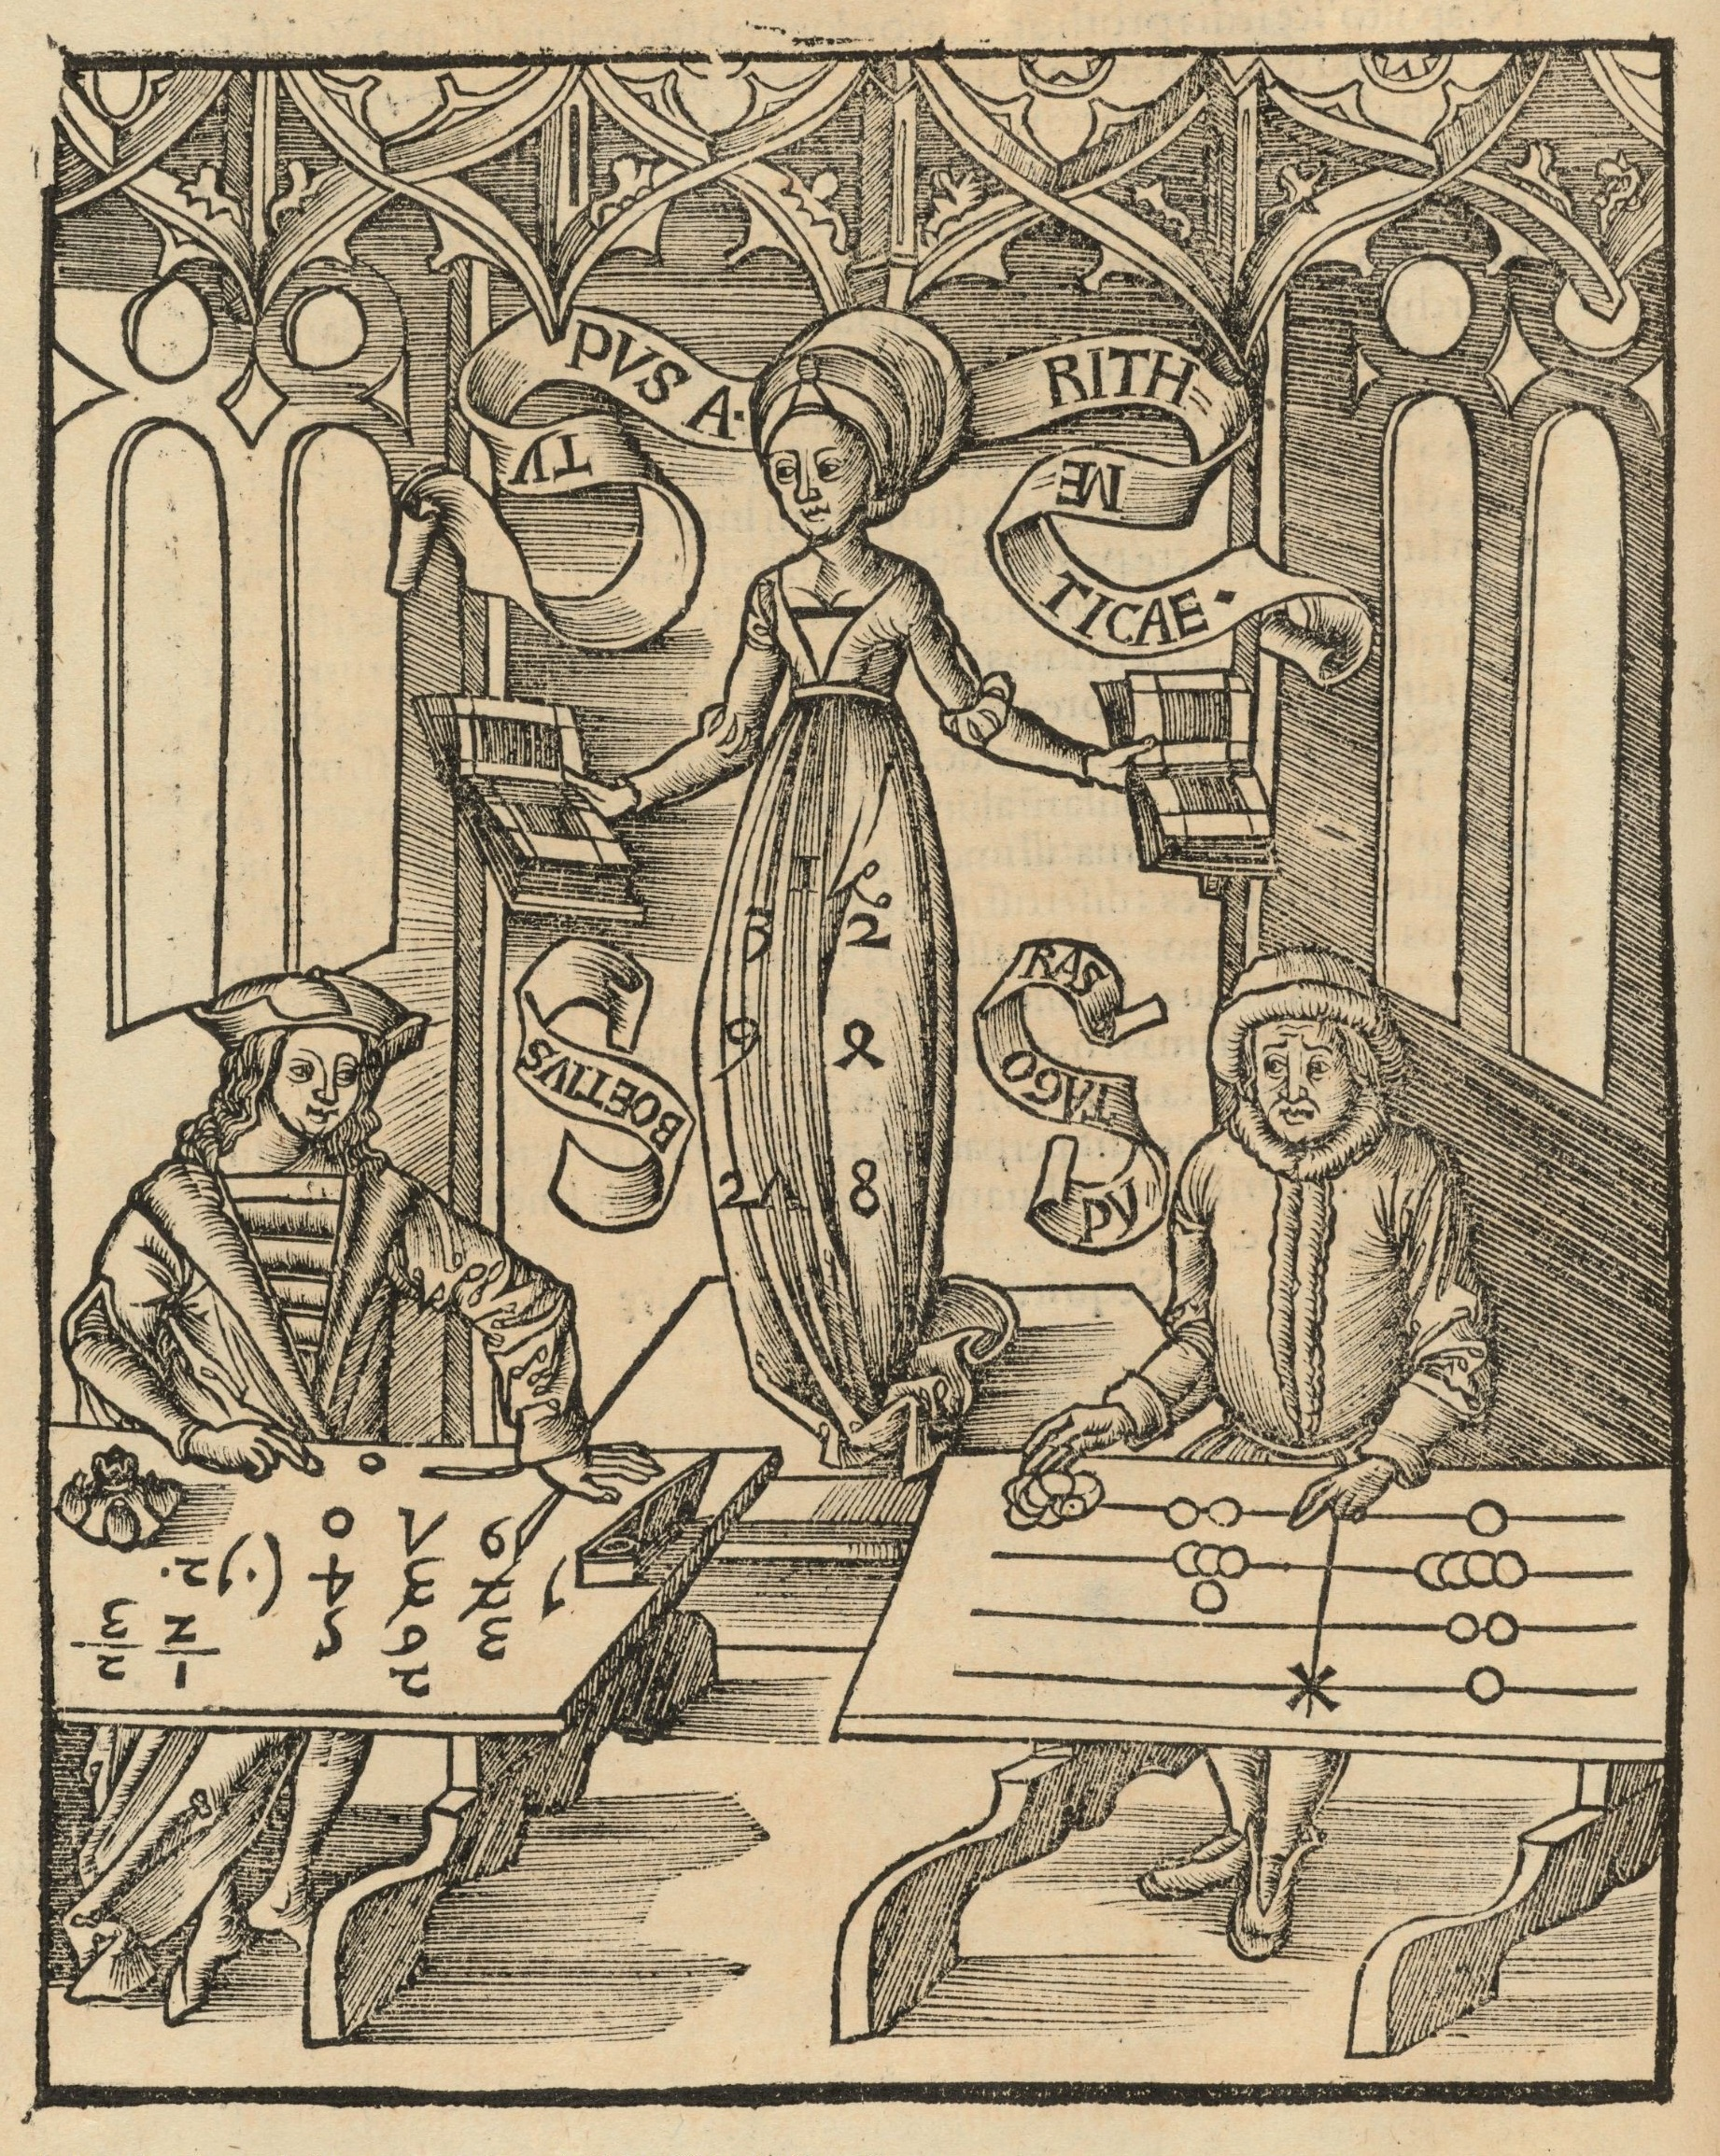
\includegraphics[width=0.4\linewidth]{algoristi_abacisti.jpg}
\end{frame}

\begin{frame}{Sistema di numerazione posizionale in base 10}
Il sistema di numerazione di tutti i giorni è un sistema \alert{posizionale} in \alert{base 10}.

Un sistema di numerazione è \alert{posizionale} quando ogni simbolo (cifra) utilizzato assume un significato diverso a seconda della posizione che occupa nella notazione.

Il rapporto fra il valore che una cifra assume in una data pozione e quella successiva è definito da una sequenza di moltiplicatori $b_1, b_2, b_3, \dots$:
\[c_4c_3c_2c_1 = c_4(b_3b_2b_1) + c_3(b_2b_1) + c_2b_1 + c_1\]
\pause
Nel caso più semplice i moltiplicatori sono tutti uguali $b_1 = b_2 = b_3 = b$ e la formula si riduce a:
\[c_4c_3c_2c_1 = c_4b^3 + c_3b^2 + c_2b + c_1\]
Il numero $b$ si chiama \alert{base} del sistema di numerazione.
\end{frame}

\begin{frame}{Codifiche in base 2, 8 e 16}
Possiamo inserire la base della codifica come pedice di un numero per indicarne la base.

Utilizzando come basi i valori 2, 8 e 16 otteniamo tre codifiche molto utilizzate in ambito informatico.

Utilizzando la formula precedente è molto semplice ricavare il valore nella base 10:

\[1234_{10} = 1\cdot10^3 + 2\cdot10^2 + 3\cdot10^1 + 4\cdot10^0 = 1234_{10}\]
\pause
\[1010_{2}  = 1\cdot2^3  + 0\cdot2^2  + 1\cdot2^1  + 0\cdot2^0 = 10_{10}\]
\pause
\[147_8 = 1\cdot8^2 + 4\cdot8^1 + 7\cdot8^0 = 103_{10}\]
\pause
\[B2A_{16} = 11\cdot16^2 + 2\cdot16^1 + 10\cdot16^0 = 2858_{10}\]
\end{frame}

\begin{frame}{Esempi conversione da base 2 a base 10}
Ricordando le potenze di 2 (1,2,4,8,16,32,64,128,...) la conversione diventa molto più facile. Basta sommare le potenze in corrispondenza degli uni:

$01101101_2 = 1+4+8+32+64 = 109_{10}$

$10010010_2 = 2+16+128 = 146_{10}$
\end{frame}


\begin{frame}{Codifica in base 2}
La codifica in base 2 (o binaria pura) è molto utilizzata in informatica perché può essere rappresentata tramite presenza o assenza di tensione elettrica.

Per passare dalla base 10 alla base 2 utilizziamo l'algoritmo delle \alert{divisioni ripetute}: dividiamo ripetutamente il numero per 2 fino ad arrivare a zero, la lettura dei resti (in ordine inverso) ci darà il numero in base 2.

\pause

	\begin{tabular}{c|c}
		\multicolumn{2}{c}{$b=2$}\\
		123 & 1 \\
		61  & 1 \\
		30  & 0 \\
		15  & 1 \\
		7   & 1 \\
		3   & 1 \\
		1	& 1	\\
		0   &  \\
	\end{tabular}
$\uparrow$
$123_{10} = 1111011_2$

In generale, dividendo ripetutamente per $b$ possiamo passare dalla base 10 alla base $b$.
\end{frame}

\begin{frame}{Codifiche in base 8 e 16}
Le basi 8 e 16 sono molto utilizzate come modo compatto per rappresentare cifre binarie.
Infatti, è molto semplice passare da base 2 a base 8 (o 16), basta tradurre a gruppi di tre (o quattro) cifre per volta partendo dalla cifra meno significativa:

\begin{tabular}{c|c}
	000 & 0 \\
	001 & 1 \\
	010 & 2 \\
	011 & 3 \\
	100 & 4 \\
	101 & 5 \\
	110	& 6	\\
	111 & 7 \\
\end{tabular}
\hspace{5cm}
\begin{tabular}{c|c}
	0000 & 0 \\
	0001 & 1 \\
	0010 & 2 \\
	0011 & 3 \\
	0100 & 4 \\
	0101 & 5 \\
	0110 & 6 \\
	0111 & 7 \\
\end{tabular}
\begin{tabular}{c|c}
	1000 & 8 \\
	1001 & 9 \\
	1010 & A \\
	1011 & B \\
	1100 & C \\
	1101 & D \\
	1110 & E \\
	1111 & F \\
\end{tabular}

\[10100101_2 = 010\ 100\ 101_2 = 245_8 \]
\[10100101_2 = 1010\ 0101_2 = A5_{16} \]
\end{frame}

\begin{frame}
\frametitle{Rappresentazione di enumerazioni}
Tramite una opportuna codifica possiamo rappresentare delle enumerazioni tramite cifre binarie.

Ad esempio, consideriamo l'insieme dei giorni della settimana. Dati $M=7$ valori distinti da rappresentare, abbiamo bisogno di $N=\ceil{\log_2 7}=\ceil{2.83}=3$ bit. 

\begin{table}[h]
	\begin{tabular}{cccc}
		lun&0&0&0\\
		mar&0&0&1\\
		mer&0&1&0\\
		gio&0&1&1\\
		ven&1&0&0\\
		sab&1&0&1\\
		dom&1&1&0
	\end{tabular}
\end{table}

Rimane una sequenza non utilizzata (111).
\end{frame}

\begin{frame}
\frametitle{ASCII}
Una delle codifiche per enumerazione più importanti è quella ASCII.

\href{https://it.wikipedia.org/wiki/ASCII}{https://it.wikipedia.org/wiki/ASCII} (notare la colonna CEC)

\begin{itemize}
\item 128 caratteri (256 ASCII esteso)
\item Caratteri di \emph{comando}, \emph{alfanumerici} e \emph{simboli}
\item Proprietà interessanti: `A' + 1 = `B' e `c' + (`A' - `a') = `C'
\end{itemize}
\end{frame}

\begin{frame}{Somme e sottrazioni in base 2}
	\begin{tabular}{r|l}
		0+0 & =0 \\
		0+1 & =1 \\
		1+0 & =1 \\
		1+1 & =0 con \alert{riporto} di 1
	\end{tabular}
\hspace{2cm}
	\begin{tabular}{r|l}
		0-0 & =0 \\
		1-0 & =1 \\
		1-1 & =0 \\
		0-1 & =1 con \alert{prestito} di 1
	\end{tabular}

\vspace{1cm}
	\begin{tabular}{r|l}
		 10 + 01 & =11 \\
		 01 + 01 & =10 \\
		 11 + 01 & =00 con \alert{overflow} \\
		 011 + 01 & =100 dopo il \alert{padding}
 	\end{tabular}
\end{frame}

\begin{frame}{Esercizi di somma}
Le somme si eseguono come in base 10. Se alla fine dell'operazione ``avanza'' un riporto, \alert{non possiamo} inserire un nuovo bit per tenerne conto, ma dobbiamo segnalare che si è verificato un \alert{overflow}, ovvero una condizione di errore.

\begin{tabular}{lr|l}
	primo operando   & 1001 & + \\
	secondo operando & 0101 & = \\
	riporti          &      &  \\
	\hline
	risultato        &   & \\
\end{tabular}
$\rightarrow$
\begin{tabular}{r|l}
	1001 & + \\
	0101 & = \\
	1\_   &   \\
	\hline
	0    &  \\
\end{tabular}
$\rightarrow$
\begin{tabular}{r|l}
	1001 & + \\
	0101 & = \\
	01\_ &   \\
	\hline
	10   &  \\
\end{tabular}

$\rightarrow$
\begin{tabular}{r|l}
	1001 & + \\
	0101 & = \\
	001\_ &   \\
	\hline
	110&  \\
\end{tabular}
$\rightarrow$
\begin{tabular}{r|l}
	1001 & + \\
	0101 & = \\
	001\_&   \\
	\hline
	1110&  \\
\end{tabular}
\end{frame}

\begin{frame}{Esercizi di somma}
\begin{tabular}{r|l}
	1101 & + \\
	0101 & = \\
	\alert{1}101\_ &   \\
	\hline
	0010& \alert{OVF}\\
\end{tabular}
\hskip 1.5cm
\begin{tabular}{r|l}
	0110 & + \\
	1010 & = \\
	\alert{1}110\_ &   \\
	\hline
	0000& \alert{OVF}\\
\end{tabular}
\hskip 1.5cm
\begin{tabular}{r|l}
	0110 & + \\
	0111 & = \\
	110\_ &   \\
	\hline
	1101& \\
\end{tabular}

\vskip 1cm
\begin{tabular}{r|l}
	10011 & + \\
	01101 & = \\
	\alert{1}1111\_ &   \\
	\hline
	00000& \alert{OVF} \\
\end{tabular}
\hskip 1.5cm
\begin{tabular}{r|l}
	010101 & + \\
	001010 & = \\
	00000\_ &   \\
	\hline
	011111& \\
\end{tabular}
\hskip 1.5cm
\begin{tabular}{r|l}
	010101 & + \\
	001111 & = \\
	11111\_ &   \\
	\hline
	100100& \\
\end{tabular}
\end{frame}

\begin{frame}{Controllo esercizi di somma}
Convertiamo le somme in base 10 per trovare eventuali errori:

\begin{itemize}
\item $1+4+16 \ \ + \ \ 1+4 = 21+5 = 26 > 2^4 \rightarrow$ \alert{OVF}
\item $2+4 \ \ + \ \ 2+8 = 6+10 = 16 = 2^4 \rightarrow$ \alert{OVF} (con 4 bit rappresentiamo 16 valori, ma considerando lo zero 16 diventa il \emph{diciassettesimo})
\item $2+4 \ \ + \ \ 1+2+4 = 6+7 = 13 = 1+4+8$
\item $1+2+16 \ \ + \ \ 1+4+8 = 19+13 = 32 = 2^5 \rightarrow$ \alert{OVF}
\item $1+4+16 \ \ + \ \ 2+8 = 21+10 = 31 = 1+2+4+8+16$
\item $1+4+16 \ \ + \ \ 1+2+4+8 = 21+15 = 36 = 4+32$
\end{itemize}
\end{frame}

\section{Numeri interi}
\begin{frame}{Notazione in modulo e segno}
Utilizzando la codifica binaria vista fin'ora, con $N$ bit possiamo rappresentare $2^N$ valori: da 0 a $2^N - 1$

Come possiamo rappresentare numeri negativi?

\pause

La notazione in modulo e segno utilizza il \alert{MSB} (most significant bit) per indicare il segno:
\[0101_2 = +101_2 = +(1+4)_{10} = +5_{10}\]
\[1101_2 = -101_2 = -(1+4)_{10} = -5_{10}\]

\pause

Con N bit useremo un bit per il segno, i rimanenti per il modulo.
Possiamo quindi rappresentare numeri nell'intervallo $-2^{N-1}+1 \leq x \leq +2^{N-1}-1$

\pause

Abbiamo infatti due possibili codifiche per il numero zero:
\[+0 = +0000 = 00000\]
\[-0 = -0000 = 10000\]
\end{frame}

\begin{frame}{Notazione in complemento alla base}
La notazione in modulo e segno spreca un valore, inoltre il calcolare avrebbe bisogno di un circuito per effettuare la somma ed un altro per effettuare la sottrazione.

La \alert{notazione in complemento alla base} risolve questi limiti: con $N$ bit ci permette di rappresentare $2^N$ valori, precisamente da $-2^{N-1}$ a $+2^{N-1}-1$.

\pause

La rappresentazione in complemento a 2, su N bit, di un numero $x_{10}$ è definita come:
\begin{itemize}
	\item $x_2$ se $x \geq 0$ (msb = 0)
	\item $(2^N-|x|)_2$ se $x < 0$ (msb = 1 in base 2, dimostrare)
\end{itemize}

\pause

Abbiamo quindi una sola rappresentazione per il numero 0.

Attenzione: il msb indica il segno solo se siamo in base 2, \alert{non è un bit di segno}.
\end{frame}


%TODO

\begin{frame}{Esempio cpl2 su 3 bit}
$N=3 \rightarrow -2^2 \leq x \leq 2^2-1 \rightarrow -4 \leq x \leq 3$
\pause

\begin{tabular}{r|l|r}
	10	&	da 10 a cpl2	&	cpl2 \\
	\hline
	+3&	1+2	&	011\\
	+2& 2	&	010\\
	+1& 1	&	001\\
	0 & 0	&	000\\
	\pause
	-1&	$2^3-|-1| = 8-1 = 7_{10} = 111_2$& 111	\\
	-2&	$8-2 = 6_{10} = 110_2$& 110	\\
	-3&	$8-3 = 5$& 101	\\
	-4&	$8-4 = 4$& 100\\
\end{tabular}

Notare che msb \alert{non è il segno}: cambiandolo non si ottiene il numero opposto.
\end{frame}

\begin{frame}{Proprietà cpl2}
Rappresentiamo un numero negativo $-x = -5$ con $N=4$ bit:\\ $-x \rightarrow (2^N-|-x|)_2 = 10000_2 - x_2 = 1111_2+1_2-x_2$

\pause
$1111-x$ possiamo ottenerlo semplicemente invertendo tutti i bit di $x$:
\begin{tabular}{r|l}
1111 & - \\
0101 & = \\
\hline
1010& \\
\end{tabular}
\hspace{2cm}
\begin{tabular}{r|l}
	1010 & + \\
	0001 & = \\
	\hline
	1011& \\
\end{tabular}

\pause
Oltre ad usare la definizione, possiamo convertire un numero negativo con questo metodo: convertire l'opposto in binario puro, invertire tutti i bit e sommare 1.

\pause
Oltre ad avvantaggiare noi umani, questa proprietà fa si che il calcolatore necessiti solo di un circuito di addizione (più quello banale di complementazione) per effettuare sia somme che sottrazioni!

\pause
Notare che invertire l'opposto e sommare 1 equivale a copiarlo da lsb a msb fino al primo 1 (compreso) ed invertire i bit rimanenti.
\end{frame}

\begin{frame}{Metodi di conversione da base 10 a cpl2}
Per convertire un numero negativo da base 10 a cpl2 abbiamo quindi tre metodi:
\begin{enumerate}[<+->]
\item Utilizzare la definizione: $(2^N-|x|)_2$:\\
$N=3; -2 \rightarrow (2^N-2)_2 = (6)_2 \rightarrow 110$
\item Convertire l'opposto in base 2, invertire i bit e sommare 1:\\
$N=3; -2 \rightarrow +2_{10} = 010_2 \rightarrow 101 \rightarrow 110$
\item Convertire l'opposto in base due, ricopiarlo da $lsb$ verso $msb$ fino al primo 1 (compreso), copiare i restanti bit complementati:\\
$N=4; -6 \rightarrow +6_{10} = 0110_2 \rightarrow 1010$
\end{enumerate}

\pause
Controlliamo l'ultimo risultato utilizzando la definizione di cpl2: $1010_2 = 2^N - |x| = 2^N+x \rightarrow x=1010_2-2^N = 10-16 = -6$

Gli stessi 3 metodi possono essere usati per convertire un numero negativo da cpl2 a base 10.
\end{frame}

\begin{frame}{Esempi di conversione da base 10 a cpl2}
Se vogliamo convertire un numero positivo lo possiamo semplicemente convertire in binario puro e poi aggiungere zeri a sinistra (padding) fino a raggiungere il numero di bit desiderati (almeno uno per il segno):
\[ 18_{10} = (16+2)_{10} = 10010_2 = 010010_2 \]

\pause
Se vogliamo convertire un numero negativo dobbiamo passare all'opposto e convertirlo in cpl2 (come sopra).
Infine dovremo complementare il risultato e sommare uno. 
Il padding verrà fatto con degli uni:
\[ -15_{10} = -(8+4+2+1)_{10} = -(1111_2) = -(01111_{cpl2}) = 10001_{cpl2} = 1110001_{cpl2} \]
\end{frame}

\begin{frame}{Esempi di conversione da cpl2 a base 10}
Se vogliamo convertire un numero da cpl2 a base 10 guardiamo il primo bit.
Se vale zero abbiamo un numero positivo e lo convertiamo come se fossimo in binario puro:
\[ 010110_{cpl2} = 2+4+16 = 22_{10} \]

\pause
Se il primo bit vale uno abbiamo invece un numero negativo, dobbiamo quindi passare all'opposto (complementando e sommando uno) e convertire in base 10 per po i passare di nuovo all'opposto:
\[1001001_{cpl2} = -(0110111_{cpl2}) = -(1+2+4+16+32) = -55_{10}\]
\end{frame}

\section{Aritmetica in complemento alla base}

\begin{frame}{Operazioni algebriche in cpl2}
Dati due numeri in base 10 da sommare algebricamente, dobbiamo innanzitutto controllare il numero di bit necessari:
\begin{itemize}
\item Se N è assegnato, dobbiamo verificare che sia sufficiente. ($-2^{N-1} \leq x \leq 2^{N-1}-1$)
\item Altrimenti dobbiamo calcolare il valore minimo capace di rappresentare \alert{entrambi} i valori.
\end{itemize}
\end{frame}

\begin{frame}{Somma senza riporto ne overflow}
Calcoliamo $-7 + 2 = -5$ con $N=4$ bit.

\pause
$-2^{N-1} = -8 \wedge 2^{N-1}-1 = +7 \rightarrow$ 4 bit sono sufficienti per rappresentare sia gli operandi che il risultato.

\pause
-7 è negativo, dunque convertiamo l'opposto (+7) in binario, poi complementiamo e sommiamo 1:
$-7 \rightarrow 7_{10} = 0111_{cpl2} \rightarrow 1001_{cpl2} = -7$

+2 è positivo, quindi lo convertiamo direttamente (con padding per avere 4 bit):
$+2 = 10_2 = 0010_{cpl2}$

\pause
Calcoliamo quindi la somma di -7 e +2:
\begin{tabular}{c|c}
$1001$ & + \\
$0010$ & = \\
\hline
$1011$& \\
\end{tabular}

Operandi discordi non possono dare overflow.

\pause
Il risultato è negativo, dunque complementiamo, sommiamo 1 e convertiamo in base 10, poi passiamo all'opposto:
$1011 < 0 \rightarrow 0101 = 5 \rightarrow -5$

$-5 = -7+2$ dunque non abbiamo fatto errori.
\end{frame}

\begin{frame}{Somma con riporto ma senza overflow}
Calcoliamo $7 - 2 = 7 + (-2) = +5$ con $N=4$ bit.

$-2^{N-1} = -8 \wedge 2^{N-1}-1 = +7 \rightarrow$ i bit sono sufficienti sia per gli operandi che per il risultato.

$+7 = 0111_2 = 0111_{cpl2}$\\
$-2 \rightarrow 2_{10} = 010_2 \rightarrow 110_{cpl2} = 1110_{cpl2} = -2$ 

\begin{tabular}{c|c}
$0111$ & + \\
$1110$ & = \\
\hline
\hskip-0.15cm\alert{1}$0101$& \\
\end{tabular}

Operandi discordi non possono dare overflow.

Ignoriamo il riporto:\\
$0101_{cpl2} = +5$
Il risultato è corretto. Quando eseguiamo operazioni in cpl2 dobbiamo sempre ignorare l'ultimo riporto.
\end{frame}

\begin{frame}{Somma senza riporto ma con overflow}
Calcoliamo $7 + 2 = +9$ con $N=4$ bit.

$-2^{N-1} = -8 \wedge 2^{N-1}-1 = +7 \rightarrow$ i bit sono sufficienti per gli operandi, ma non per il risultato: ci aspettiamo una situazione di overflow.

$+7 = 0111_2 = 0111_{cpl2}$\\
$+2 = 0010_2 = 0010_{cpl2}$

\pause
\begin{tabular}{c|c}
$0111$ & + \\
$0010$ & = \\
\hline
$1001$& \\
\end{tabular}

\pause
$1001_2$ è un numero negativo, dunque passiamo all'opposto $0111_{cpl2}$, che convertito in base 10 vale $1+2+4=7$, dunque il risultato vale -7 ed è sbagliato (coerentemente con la situazione di overflow).

Non abbiamo riporto, cosa ci indica la presenza di overflow?
\pause
Gli operandi sono concordi fra loro ma discordi dal risultato, dunque si è verificato overflow.
\end{frame}

\begin{frame}{Somma con riporto e overflow}
Calcoliamo $(-7) + (-2) = -9$ con $N=4$ bit.

$-2^{N-1} = -8 \wedge 2^{N-1}-1 = +7 \rightarrow$ i bit sono sufficienti per gli operandi, ma non per il risultato e avremo una situazione di overflow.

$-7 \rightarrow 7_{10} = 0111_2 \rightarrow 1001_{cpl2}$\\
$-2 \rightarrow 2_{10} = 0010_2 \rightarrow 1110_{cpl2}$

\begin{tabular}{c|c}
$1001$ & + \\
$1110$ & = \\
\hline
\hskip-0.15cm\alert{1}$0111$& \\
\end{tabular}

Ignoriamo il riporto:
$0111 > 0 \rightarrow 0111 = 7 \rightarrow +7$

Operandi concordi ma risultato discorde indicano che siamo in una condizione di overflow.
(Operandi discordi non daranno mai overflow)
\end{frame}

\section{Esercizi da TdE}

\begin{frame}{Esercizio completo - TdE 10/09/2018}
\begin{enumerate}
	\item Si dica quale dei seguenti cinque numeri è il maggiore motivando la risposta:
	\begin{itemize}
		\item 34 in base 8;
		\item 34 in base 10;
		\item 0A1 in base 16;
		\item 1111111 in Complemento a 2;
		\item 0011011 in Complemento a 2.
	\end{itemize}
	
	\item Si indichi quindi il numero n di bit che permette di codificare tutti i numeri A - E in Complemento a 2 e li si codifichi tutti in Complemento a 2 usando n bit, riportando i passaggi fondamentali dei calcoli.
	
	\item Si eseguano (riportando i calcoli) le seguenti operazioni utilizzando n bit e si indichino eventuali bit di carry (riporto) e overflow:
	\begin{itemize}
		\item A - B;
		\item C + B + E.
	\end{itemize}
\end{enumerate}
\end{frame}

\begin{frame}{TdE 10/09/2018 - Soluzione punto 1}
Convertiamo tutti i valori in base 10.
	\begin{itemize}
		\item $34_8 = 3 \cdot 8 +  4 = 24+4 = 28_{10}$
		\item $34_{10}$
		\item $0A1_{16} = 10 \cdot 16 + 1 = 161_{10}$
		\item $1111111_{cpl2}$ è negativo, passiamo all'opposto e convertiamolo: $0000001_2 = 1_{10}$, dunque il numero vale -1
		\item $0011011_{cpl2}$ è positivo, lo convertiamo direttamente: $0011011_2 = 1+2+8+16 = 27_{10}$
	\end{itemize}

Dunque il maggiore è $0A1_{16}$.

Notare che non era necessario convertire tutti i numeri: A è minore di B per la base e D è negativo.
\end{frame}

\begin{frame}{TdE 10/09/2018 - Soluzione punto 2 - numero di bit necessari}
Con $N$ bit possiamo rappresentare da $-2^{N-1}$ a $2^{N-1}-1$.

\pause

Per il numero minore (-1) basterebbero solo 2 bit, controlliamo dunque il maggiore, sapendo che ci servono almeno 5 bit (ultimo numero):

\pause
\begin{center}
\begin{tabular}{ccc}
	$N$	&	min	&	max	\\
	\hline
	5	&	-16	&	15	\\
	6	&	-32	&	31	\\
	7	&	-64	&	63	\\
	8	&	-128&	127	\\
	9	&	-256&	255 \\
\end{tabular}
\end{center}

Dunque ci servono 9 bit.
\end{frame}

\begin{frame}{TdE 10/09/2018 - Soluzione punto 2 - conversione}
Convertiamo i primi 3 numeri con il metodo delle divisioni ripetute (o con le tabelle per base 8 e 16) e aggiungendo zeri a sinistra fino ad arrivare a 9 bit:
	\begin{itemize}
		\item $34_8 = 000\ 011\ 100_{cpl2}$
		\item $34_{10} = 000100010_{cpl2}$
		\item $0A1_{16} = 0\ 1010\ 0001_{cpl2}$
	\end{itemize}

\pause
Per gli ultimi due numeri aggiungiamo uni o zeri a sinistra fino ad arrivare a 9 bit:
	\begin{itemize}
		\item $1111111_{cpl2} = 111111111_{cpl2}$
		\item $0011011_{cpl2} = 000011011_{cpl2}$
 	\end{itemize}
\end{frame}

\begin{frame}{TdE 10/09/2018 - Soluzione punto 3 - $A-B$}
$A-B = A + (-B)$ dunque troviamo $-B = 111011110_{cpl2}$

\pause
\begin{tabular}{r|l}
	000 011 100 & + \\
	111 011 110 & = \\
	\hline
	000 111 00\_&	riporti\\
	111 111 010	& risultato
\end{tabular}

\pause
Operandi discordi non possono dare overflow.

\pause
Controlliamo il risultato: $111111010 _{cpl2}$ è negativo, quindi convertiamo l'opposto.
$000000110_2 = 2+4 = 6_{10}$

Dunque il risultato vale -6, che è corretto: $A-B = 28-34 = -6$

\end{frame}

\begin{frame}{TdE 10/09/2018 - Soluzione punto 3 - $C+B+E$}
\begin{tabular}{r|l}
	010 100 001 & + \\
	000 100 010 & + \\
	000 011 011 &	=	\\
	\hline
	001 000 11\_&	riporti\\
	011 011 110	& risultato
\end{tabular}

\pause
Gli operandi sono concordi con il risultato, dunque non si è verificato overflow.

\pause
Convertiamo il risultato in base 10: $011011110_2 = 2+4+8+16+64+128 = 222_{10} = 161+34+27$
\end{frame}

\begin{frame}{Esercizio a 10 bit}
Calcoliamo il risultato di 324 - 413.

\pause
$-413_{10} = -(110011101_2) = -(0110011101_{cpl2}) = 1001100011_{cpl2}$\\
$324_{10} = 101000100_2 = 0101000100_{cpl2}        = 0101000100_{cpl2}$

\pause
\begin{tabular}{r|l}
	1 001 100 011 & + \\
	0 101 000 100 & = \\
	\hline
	0 010 000 00\_&	riporti\\
    1 110 100 111 & risultato
\end{tabular}

\pause
Risultati discordi non danno overflow.

\pause
$1110100111_{cpl2} = -(0001011001_{cpl2}) = -(1+8+16+64)_{10} = -89_{10} = 324-413$
\end{frame}



\begin{frame}{Esercizio somma}
Si scriva la codifica in complemento a due dei numeri $a=-68$ e $b=+73$ utilizzando 8 bit.
Calcolare inoltre il risultato di $a-b$ e commentarlo.
\end{frame}

\begin{frame}{Esercizio somma - Soluzione 1}
\begin{itemize}[<+->]
\item Con 8 bit rappresento da $-2^{8-1} = -128$ a $+2^{8-1}-1 = +127$. Posso rappresentare gli operandi.
\item $(-68) - (+73) = (-68) + (-73) = -141$ Non posso rappresentare il risultato, mi aspetto overflow.
\item $-68 < 0 \rightarrow$ passo all'opposto, converto in base 2, copio da lsb a msb fino al primo uno poi complemento $\rightarrow 68_{10} = 1000100_2 = 01000100_2 \rightarrow 10111100$
\item $-73 < 0 \rightarrow 73_{10} = 1001001_2 = 01001001_2 \rightarrow 10110111$
\end{itemize}
\end{frame}

\begin{frame}{Esercizio somma - Soluzione 2}
\begin{tabular}{c|c}
$10111100$ & + \\
$10110111$ & = \\
\hline
\hskip-0.15cm\alert{1}$01110011$& \\
\end{tabular}

Ignoro il riporto e considero $01110011$, operandi concordi danno risultato discorde, si è verificato overflow.

Infatti, se converto $01110011$ ottengo $1+2+16+32+64 = 115$ (nota che $115+141=256=2^8$)
\end{frame}



\begin{frame}[allowframebreaks]{TdE 26 Giugno 2017}
Si  dica  e  si  motivi  qual  è  il  minimo  numero  di  bit  che  permette  di  rappresentare  in  
complemento  a  due  (CP2)  tutti  i  numeri  seguenti:  
\begin{enumerate}
	\item A  =  +  255  
	\item B  =  -­  42  
	\item C  =  +  7  
	\item D  =  -­  257  
\end{enumerate}

\framebreak
Se  si  volessero  eseguire  tutte  le  possibili  somme  e  sottrazioni  tra  le  coppie  di  numeri  A,  B,  
C,  D,  qual  è  il  minimo  numero  di  bit  in  cui  dovrebbero  essere  rappresentati  i  numeri?  Si  
motivi  la  risposta

Si  calcoli  il  risultato  dell’operazione  7  -­  255  utilizzando  la  rappresentazione  in  CP2  con  il  
numero  di  bit  stabilito  nel  punto  (a).  Si  mostrino  tutti  i  passaggi  eseguiti  e  si  indichino  i  bit  di  
carry  e  di  overflow.
\end{frame}

\begin{frame}[allowframebreaks, fragile]{TdE 26 Giugno 2017 - Soluzione}
In CP2 con $n$ bit posso rappresentare da $-2^{n-1}$ a $2^{n-1}-1$.

Dato un numero negativo $x$ mi serviranno dunque $n = \log_2{-x}+1$ bit per rappresentarlo e dato un numero positivo $y$ me ne serviranno $n = \log_2(y+1)+1$

Le potenze di 2 sono: 1 2 4 8 16 32 64 128 256 512 ...

I due numeri che devo controllare sono A e D:
\begin{itemize}
\item A=255 $\rightarrow$ $n_A = \log_2{256}+1 = 9$
\item D=-257 $\rightarrow$ $n_B = \log_2{257}+1 = 10$
\end{itemize}

Dunque mi servono \alert{10 bit} per rappresentare tutti i valori.

\framebreak

Le operazioni che possono dare problemi sono le sottrazioni che coinvolgono A e D. In particolare, A-D darà un numero positivo, mentre D-A darà un numero negativo. Le due operazioni avranno risultato uguale in valore assoluto. Dato che con $n$ bit posso rappresentare da $-2^{n-1}$ a $2^{n-1}\alert{-1}$ controllo solo A-D che dando un risultato positivo è l'operazione più problematica a causa del \alert{-1}.

$A-D=255-(-257) = 255+257 = 256+256 = 512 = 2^9$ e per rappresentarlo mi servono $n = \log_2(2^9+1)+1 = 10+1 = 11$.

Mi servono dunque 11 bit per eseguire tutte le possibili somme e sottrazioni.

\framebreak

Converto +7 in CPL2. Inizio a convertirlo in base 2:
\begin{tabular}{c|c}
7 & 1\\
3 & 1\\
1 & 1\\
0 & 
\end{tabular}\\
La rappresentazione è dunque 111. Essendo un numero positivo la notazione in CPL2 è 0111. Dovendo usare 10 bit aggiungo degli zeri a sinistra: 0000000111

\framebreak
Inizio a convertire +255 in base 2:
\begin{tabular}{c|c}
255 & 1\\
127 & 1\\
63 & 1\\
31 & 1\\
15 & 1\\
7 & 1\\
3 & 1\\
1 & 1\\
0 & 
\end{tabular}\\
La rappresentazione di +255 è dunque 11111111. Aggiungo uno 0 a sinistra per avere la rappresentazione in CPL2: 011111111. Noi siamo interessati a -255, dunque copiamo da sx verso dx fino al primo 1 compreso, poi complementiamo: 100000001 e aggiungiamo degli 1 a sinistra per ottenere 10 bit: 1100000001

\framebreak

\begin{tabular}{cc|c}
7			& 0000000111 & + \\
-255		& 1100000001 & = \\
riporti		& \ \ \ \ \ \ \ \ 111\ &  \\
\hline
risultato	& 1100001000 &  \\
\end{tabular}

Operandi discordi non possono dare overflow.

Controllo il risultato: 1100001000 è negativo, l'opposto è 0011111000, che vale $8+16+32+64+128 = 248 \rightarrow -248 = -255+7$

\end{frame}

\begin{frame}{Esercizio somma}
Si considerino $A_{10} = +77$ e $B_{CPL2} = 101110$ (già in complemento a 2). Li si rappresenti entrambi in base 2 notazione complemento a 2, sul numero \alert{minimo} di bit per rappresentare \alert{entrambi} gli operandi. Si effettuino quindi, sul numero di bit prima individuato, le
operazioni A+B e A–B in complemento a 2, indicando se si verifica overflow oppure no.
\end{frame}

\begin{frame}[allowframebreaks]{Esercizio somma - soluzione}
\begin{tabular}{c|c}
77 & 1\\
38 & 0\\
19 & 1\\
9 & 1\\
4 & 0\\
2 & 0\\
1 & 1\\
0 &
\end{tabular}
$77_{10} = 1001101_2 = 01001101_{CPL2}$

Ho rappresentato $A$ con 8 bit, devo aggiungere 2 bit a B. Essendo B negativo (inizia con 1) aggiungo degli 1: $B=11101110_{CPL2}$

Noto anche che B vale -18, in quanto: $-B=010010_2=16+2=18_{10}$

\framebreak
Eseguo A+B

\begin{tabular}{cc|c}
A			& 01001101 & + \\
B			& 11101110 & = \\
\hline
risultato	&\hspace{-0.5cm}(1)00111011 &  \\
\end{tabular}

Ignoro il riporto. Il risultato è 00111011. Operandi discordi non possono dare overflow.
$00111011 = 1+2+8+16+32=59=77-18$

\framebreak

Eseguo A-B = A+(-B).\\
$-B = 00010010_{CPL2}$

\begin{tabular}{cc|c}
A			& 01001101 & + \\
-B			& 00010010 & = \\
\hline
risultato	& 01011111 &  \\
\end{tabular}

Operandi concordi hanno dato un risultato ad essi concorde, quindi non si è verificato overflow.

$01011111 = 1+2+4+8+16+64=95=75-(-18)$

\end{frame}


\end{document}